% Online sync refresh: revised workshop report, 2026-08-29. figure-path-fix
To investigate whether UCB learns the true value of each arm, the algorithm
was simulated for \(T=10^4\) steps over \(M=300\) independent reruns for
\(c\in\{0,1,2\}\). Each arm was selected once initially to avoid an undefined
confidence bonus. Thereafter, actions were selected using the UCB rule and
the empirical action-value estimate \(Q_t(a)\) was updated by the sample
average.

Since the true values \(q^\ast(a)\) are known in the simulated environment,
the estimation accuracy of each arm was measured using
\[
    \operatorname{RMSE}_t(a)
    =
    \sqrt{
        \frac{1}{M}
        \sum_{r=1}^{M}
        \left(
            Q_t^{(r)}(a)-q^\ast(a)
        \right)^2
    }.
\]
A decreasing RMSE therefore indicates that the empirical estimate of an arm
is approaching its true value.

\begin{figure}[H]
    \centering
    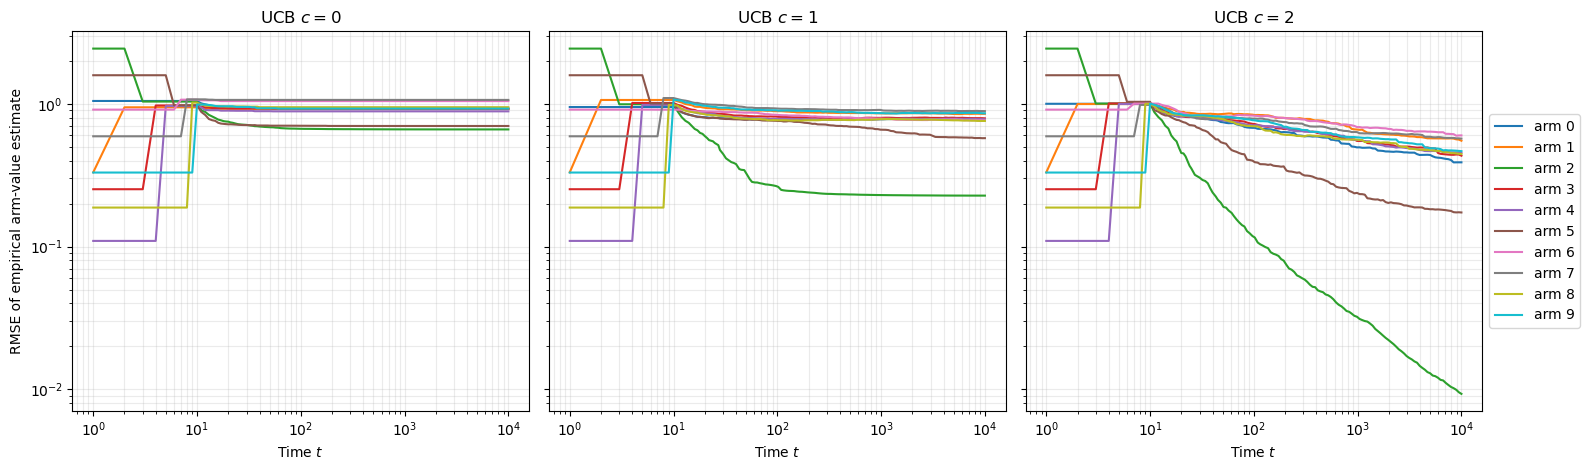
\includegraphics[width=\linewidth]
    {figures/q4_ucb_arm_value_rmse.png}
    \caption{RMSE of the empirical value estimate for each arm under UCB
    with \(c=0,1,2\), averaged over \(300\) independent reruns.}
    \label{fig:q4-ucb-rmse}
\end{figure}

As shown in Figure~\ref{fig:q4-ucb-rmse}, the amount of exploration has a
strong effect on value estimation. For \(c=0\), the confidence bonus
vanishes and the algorithm becomes purely greedy after the initial pulls.
Consequently, many arms are never revisited and their estimation errors do
not decrease. The final mean arm-wise RMSE is approximately \(0.898\).

For \(c=1\), UCB continues to revisit uncertain arms, reducing the final mean
arm-wise RMSE to approximately \(0.725\). However, highly suboptimal arms
are sampled only a few times by \(T=10^4\), so their estimates remain noisy.
Increasing the exploration coefficient to \(c=2\) produces substantially more
accurate estimates across the arms, reducing the final mean arm-wise RMSE to
approximately \(0.409\).

At the finite horizon $T=10^4$, $c=2$ therefore gives substantially better
arm-value estimation, while $c=1$ still leaves several poor arms sparsely
sampled and has not accurately learned every arm. Asymptotically, if an
arm's count remained bounded while time increased, its bonus
$c\sqrt{\log(t+1)/N_t(a)}$ would diverge and force that arm to be revisited.
Thus exploratory UCB supports eventual learning of every arm, but the
numerical results show that this can be extremely slow for highly
suboptimal arms. The degenerate case $c=0$ does not in general learn every
arm because it ceases systematic exploration.
